\subsection{Needle variations}
We introduced a tool to describe variations of trajectories. Now we are going to analyze a way of causing trajectory variations. This will be of made with control variations, not through the variation of initial conditions.


\paragraph{Needle variation (fixed interval)}
Let \controlSystem\space be a control system, $x_0\in\chi$ be an initial condition for eq. \eqref{e1.1}, $\tzto\subset\R$ a time interval, $\mu\in\admContr{x_0,t_0,\tzto}$. We then define 
\lista{
	\item the \grass{fixed interval needle variation data} as a triple $\theta=(\tau_\theta,l_\theta,\omega_\theta)$ for which \lista{
		\item $\tau_\theta\in(t_0,t_1]$,
		\item $l_\theta\in\R_{\geq0}$,
		\item $\omega_\theta\in U$.
	}

	\item the \grass{control variation} of the control $\mu$ associated to the relative fixed interval needle variation data $\theta$ is the map $\mu_\theta:J\times\tzto\fd U$ such that
	\[\mu_\theta = \left\{ \begin{array}{lr}
	\omega_\theta & \mbox{if $t\in[\tau_\theta-sl_\theta,\tau_\theta]$}\\
	\mut & \mbox{otherwise}.\end{array}
	\right.	\]
	Where $J=[0,s_0]$ is an interval sufficiently small so that $\mu_\theta(s,t)$ is an admissible control for each $s\in J$.
	Just to have an idea, this is how the function $\mu_\theta$ can look like for a certain $s>0$.
	\begin{figure}[H]
		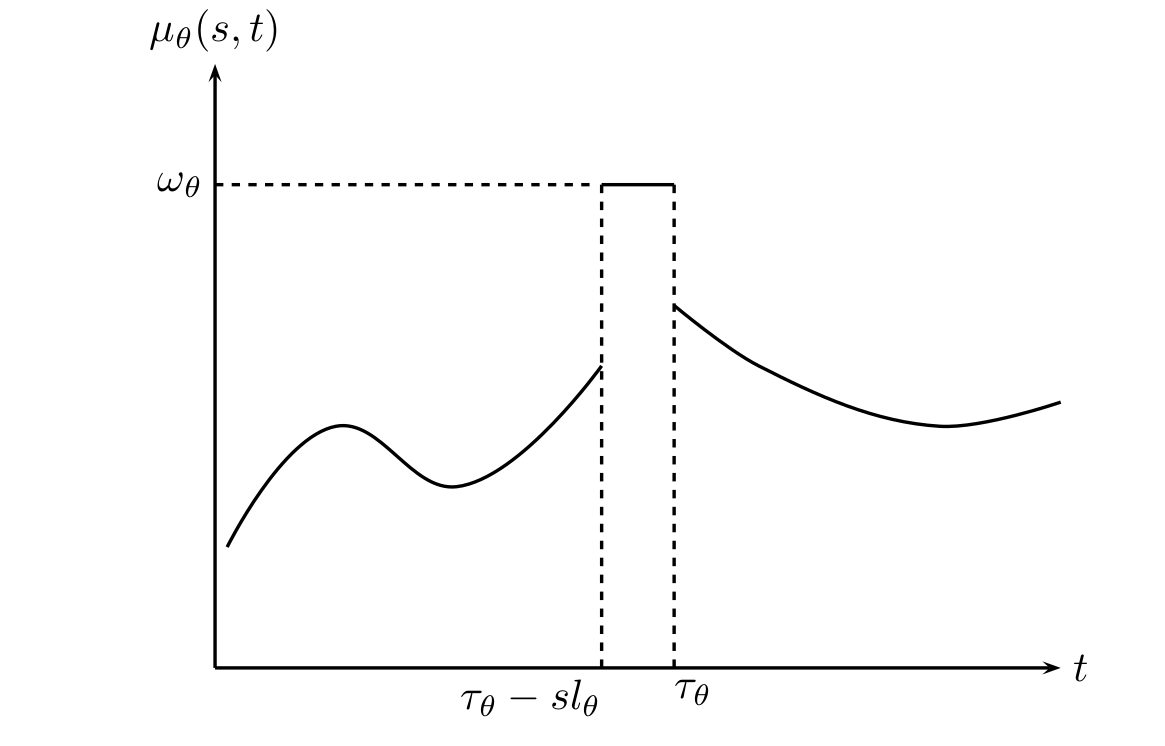
\includegraphics[width=\linewidth]{imgs/needle-variation.png}
		\caption{}
		\label{fig-needle-variation}
	\end{figure}
	\item the \grass{fixed interval needle (infinitesimal) variation} associated with the control $\mu$, the trajectory \trajWinCond{\cdot} and the variation data $\theta$ as the vector of $\R^n$ defined as 
	\[v_\theta = \frac{d}{ds}\bigg|_{s=0} \xi(\mu_\theta(s,\cdot),x_0,t_0,\tau_\theta),\] when such derivative exists.
}
This limit exists at almost any instant, as the next theorem says. Before though we need the definition of $Leb(\mu,x_0,t_0,t)$: it's the set of Lebesgue points of $\tau\fd f(\trajWinCondMath{\tau},\mu(\tau))$ in the interval $(t_0,t)$.

\paragraph[prop 4.9]{Existence and form of fixed interval needle variations}
\begin{teo}
	 Let \controlSystem\space be a control system, $x_0\in\chi$ be an initial condition for eq. \eqref{e1.1}, $\tzto\subset\R$ a time interval, $\mu\in\admContr{x_0,t_0,\tzto}$. Let then $\theta=(\tau_\theta,l_\theta,\omega_\theta)$ be a fixed interval needle variation data, with $\tau_\theta\in Leb(\mu,x_0,t_0,t_1)$. Then the fixed interval variation associated with those data exists and it's given by
\[ v_\theta=l_\theta*\bigg(f(\trajWinCondMath{\tau_\theta},\omega_\theta) - f(\trajWinCondMath{\tau_\theta},\mu(\tau_\theta) )  \bigg). \]
	\label{4-9}
	\label{T5}
\end{teo}

\subparagraph[4.10]{Variations and cones} The real importance of this theorem is not only in the fact that it is (almost) always possible to individuate the infinitesimal variation, but also in the fact that those variations form a cone, which is, if one vector represents a variation, then all of the half-line (originating from $0\in\R^n$) given by that vector is made up of fixed interval variations. Formally said: \\

\begin{teo}
	Let \controlSystem\space be a control system, $x_0\in\chi$ be an initial condition for eq. \eqref{e1.1}, $\tzto\subset\R$ a time interval, $\mu\in\admContr{x_0,t_0,\tzto}$. Let then \fivData\space be a fixed interval needle variation data, with $\tau_\theta\in Leb(\mu,x_0,t_0,t_1)$.\\
Then, the set of fixed interval needle variation associated with the data $\theta$ form a cone.
	\label{4-10}
	\label{T6}
\end{teo}
\begin{proof}
	It's just enough to say that, if $v_\theta$ is the variation associated with the data \fivData, then, taken a $k\in\R_{\geq0}, kv_\theta$ is the variation associated with the data $k\theta=(\tau_\theta,kl_\theta,\omega_\theta)$. Using obvious notation, one could then say that $v_{k\theta}=kv_\theta$.
\end{proof}
It is interesting to note that, in the triple representing the data, only the "lenght of the disturbance" gets multiplied by the scalar. This means, that, referring to Figure \ref{fig-needle-variation}, only the length of the horizontal step in the figure changes. But in the limit process the disturbance is reduced to a 0-measure point, regardless of its underlying $l_\theta$.\\
The only effect one may obtain is that, given a certain trajectory, the trajectories associated with varied control depart from the undisturbed one at a higher rate with growing s (at least, as long as s is small enough so that one can linearize the effect of control variation), but in the same direction (this is exactly the same concept as the cone).

%\subsection{Multi-needle variations}
%The concept behind multi needle variations is that they are made of single needle variations which sum up(linearly, as can be see in the relative theorem). We need this object basically because although single needle variations do form a cone, this is not generally convex. Convexity is needed in the proof, to find a hyperplane that separates the half space containing cone from another one. This is because a variational cone originating from the boundary of the reachable set cone will point toward the "less optimal", this half space is the non optimal one.\\\\
%So now let \controlSystem be a control system, $x_0\in\chi$ be an initial condition for eq. \ref{e1.1}, $\tzto\subset\R$ a time interval, $\mu\in\admContr{x_0,t_0,\tzto}$. We want to define
% \lista{
%	\item the \grass{fixed interval multi-needle variation data $\Theta$} as the collection $\Theta=\{\theta_1,..,\theta_k\}$ of fixed interval needle variation data $\theta_j=(\tau_j,l_j,\omega_j),j=1,..,k$, with the times $\tau_j$ all distinct.
%	
%	\item the \grass{control variation} of the control $\mu$ associated with the relative data $\Theta$ as the map $\mu_\Theta:J\times\tzto\fd U$ such that
%	\[\mu_\Theta = \left\{ \begin{array}{ll}
%	\omega_j & \mbox{if $t\in[\tau_\Theta-sl_\Theta,\tau_\Theta],j=1,..,k$}\\
%	\mut & \mbox{otherwise}.\end{array}
%	\right.	\]
%	Where $J=[0,s_0]$ is an interval sufficiently small so that $\mu_\Theta(s,t)$ is an admissible control for each $s\in J$.
%	
%	\item the \grass{fixed interval multi-needle variation} associated with the control $\mu$, the trajectory \trajWinCond{\cdot}, the time $t\in\tzto$ taken such that $t>\underset{j}{\max}(\tau_j)$ and the variation data $\Theta$ as a vector of $\R^n$ (a vectorial function of time actually) defined like this: 
%	\[v_\theta(t) = \frac{d}{ds}\bigg|_{s=0} \xi(\mu_\Theta(s,\cdot),x_0,t_0,t),\] when such derivative exists.
%}
%
%\paragraph[4.12]{Existence of multi-needle fixed interval variations}\mbox{}\\
%\begin{teo}
%	Let \controlSystem\space be a control system, $x_0\in\chi$ be an initial condition for eq. \eqref{e1.1}, $\tzto\subset\R$ a time interval, $\mu\in\admContr{x_0,t_0,\tzto}$. Then, let $\Theta=\{\theta_1,..,\theta_k\}$ be a multi needle variation data ("fixed interval" will from now on be omitted, since this case is the only one treated in this essay). $\Theta$ is such that the times $\tau_j\in Leb(\mu,x_0,t_0,t)$, are all distinct, and also $t>\underset{j}{\max}(\tau_j)$.\\
%Then, the multi needle variation is given by
%\[v_\Theta(t)=\sum_{j=1}^{k}\fondMatMath{\tau_j}{t}\cdot v_{\theta_j} \]
%\label{4-12}
%\end{teo}
%As one can see, the variations caused by the various single needle variations are first evolved in time from the instant in which they are applied to the "current" one, $t$, and then their effects sum up linearly.\\\\
%Taking this into account, and also considering the fact that $v_{k\theta_j}=kv_{\theta_j}$ for whatever $k\geq0$ real, and remembering that the matrix-vector product is linear with respect to scalar multiplication, one can easily get the following
%\subparagraph[4.13]{Coned convex combination of multi needle variations} 
%\begin{cor}
%	With slight abuse of notation, consider the usual control system, admissible control, initial condition, interval. Given a multi needle variation data with its distinct times being Lebesgue points for $f$, and with a $t>\underset{j}{\max}(\tau_j)$, given a set $\lambda=\{\lambda_1,..,\lambda_k\}\subset\R_{\geq0}$ then
%\[ v_{\lambda\Theta(t)}=\sum_{j=1}^{k}\lambda_j\fondMatMath{\tau_j}{t}\cdot v_{\theta_j}. \]
%\label{4-13}
%\end{cor}

\subsection{The tangent cone}
The proof of maximum principle will make use of cones of variations and relate them to the reachable set. \\

%The variations used will be both single and multi needle. We're going to see that the two are, in a sense, equal.\\ We just need two more definitions.\\ 
%\paragraph{Tangent cone}
As usual, let \controlSystem\space be a control system, $x_0\in\chi$ be an initial condition for eq. \eqref{e1.1}, $\tzto\subset\R$ a time interval, $\mu\in\admContr{x_0,t_0,\tzto}$. We then take $t\in\tzto$. Then we denote with \fixIntTanCone{t} the coned convex hull of the following set: 
\[ \cup \{ \fondMatMath{\tau}{t}\cdot v|\tau\in Leb(\mu,x_0,t_0,t)\text{where $v$ is a single needle variation at time }\tau. \} \]
This cone will be called \grass{tangent cone}.\\
In simple words, $K$ is built by taking every single needle variation at every possible time preceding the current one(almost: they still have to be Lebesgue points), making the disturbance evolve from its origin to the current time trough matrix $\Phi$ and then by taking the coned convex hull of the set union of all those vectors. \\
%We now define the analogue to \fixIntTanCone{t} but for multi needle variations.
%
%\paragraph{Tangent r-simplex cone(and relative data)} As usual, let \controlSystem\space be a control system, $x_0\in\chi$ be an initial condition for eq. \eqref{e1.1}, $\tzto\subset\R$ a time interval, $\mu\in\admContr{x_0,t_0,\tzto}$. We then take $t\in\tzto$. We have the following definitions: 
%\lista{
%	\item \grass{tangent r-simplex cone data} as a collection $\{\Theta_1,...,\Theta_r\}$ of multi needle variations. \\
%	We use this notation:$\Theta_i=\{\theta_ij\};i=1,..,r;j=1,..,k_i$,and require that the times $\tau_ij$ are all distinct and that they are all Lebesgue points.
%	
%	\item given the multi needle variations $v_{\Theta_i}$associated with the relativa r-simplex cone data, the coned convex hull of $v_{\Theta_i}$  is actually an r-simplex cone and defined as the \grass{tangent r-simplex cone}. 
%}
%Of course, when not explicitly said, the previous definitions where all relative to the fixed-interval case.
%
%\paragraph[lemma 5.5]{Various forms for the tangent cone}
%\begin{teo}
%	The following sets are actually the same set: \lista{
%	\item \fixIntTanCone{t}.
%	\item given r=$dim(\fixIntTanConeMath{t})$, the closure of the set formed by the union of all the possible tangent r-simplex cones.
%	\item the closure of the set formed by the union of all the sets $\{\fondMatMath{\tau}{t}\cdot\fixIntTanConeMath{\tau}| \tau\in Leb(\mu,x_0,t_0,t)\}$.
%}
%\label{5-5}
%\end{teo}
%Despite the difficulty of interpretation, this theorem tells us that in the end it does not matter if variations to the control are obtained through single needle or multi needle variations. The equivalence of the first one and the third one is easier to justify and understand, using the property of concatenation of $\Phi$ for which $\fondMatMath{a}{b}\cdot\fondMatMath{b}{c}=\fondMatMath{a}{c}$.
%
\subsection{Significative theorems}
\paragraph[5.10]{Points in the tangent cones are "interior" to the reachable set}
\begin{teo}
	Given the usual control system, initial condition and $\tzto$, and given a tangent cone \fixIntTanCone{t}, for a $t\in\tzto$, if a $v_0$ exists such that it is in the internal part of $K$,then there exists a cone $A\subset int(K)$ and an $r>0$ such that \lista{
\item $v_0\in int(A)$,
\item the intersection B between A and the ball of center \trajWinCond{t}  and radius r is contained in the reachable set $B\subset$\reachSet{t}. In other words, \reachSet{t}$\supset B=\{\trajWinCondMath{t} +v| \text{\space}v \in A,||v||<r \}$}
\label{5-10}
\label{T7}
\end{teo}

What this theorem says is that basically the tangent cone points "towards", or better to say, "in" the reachable set. 

\paragraph[5.12-5.14]{Maximum Hamiltonians and tangent cones}
In the statement of maximum principle tangent cones do not appear, but maximum Hamiltonian do. Actually, one could just be satisfied with the Hamiltonian part, in the sense that, once the adjoint response is found (not an easy task, but the orthogonality with the smooth set \so\space and \sz\space can help), the only remaining part is to find controls that maximizes the Hamiltonian. Only those controls are candidates for optimality. 

Nevertheless, it is interesting to see the connections between tangent cones and Hamiltonians, and to have a look at the (geometrical) significance of the following theorems.\\
The first one is going to be about the binding between maximization of Hamiltonian and the existance of a separating hyperplane between the costate and, in a sense, possible "force fields". This, point to point in time. 

\begin{teo}
Given a control system \controlSystem, a costate $p$ and a control $\overline{u}$, then\\
$H_\Sigma(x,p,\overline{u})=H_{\Sigma}^{max}(x,p)$ if and only if 
\[ \text{for every }v\in\{f(x,u)-f(x,\overline{u})|u\in U \}\text{ it is valid that }\langle p,v \rangle\le0 \]
\label{T8}
\label{5-12}
\end{teo}

\begin{proof}
	\begin{gather*}
	H_\Sigma(x,p,\overline{u})=H_{\Sigma}^{max}(x,p) \iff\\
	H_\Sigma(x,p,\overline{u})\ge H_\Sigma(x,p,u) \iff \\
	H_\Sigma(x,p,\overline{u})- H_\Sigma(x,p,u) \ge0 \iff\\
	\langle p,f(x,u)-f(x,\overline{u}) \le 0\rangle \iff\\
	\langle p,v \rangle \leq 0
\end{gather*}
for $v$ defined as before.
\end{proof}


\paragraph[5.13]{Hamiltonians and adjoint response}
There is now another theorem, regarding the connection between adjoint response and Hamiltonian. What this theorem says is that one can find a suitable costate $p$, which maximizes the Hamiltonian up to the present moment.
 \begin{teo}
 	Let's have the usual control system, initial condition, time interval, and suppose that for a $\tau\in\tzto$ there exists a vector $\overline{\lambda}\in\R^n$ ad a cone A, such that $\fixIntTanConeMath{\tau}\subset A$ and  for each $v\in A \implies \langle \overline{\lambda},v\rangle\leq0$. If we then take the adjoint response with initial condition for equation \eqref{adjoint-equation} that $\lambda(\tau)=\overline{\lambda}$ it holds true that for every $t\in Leb(\mu,x_0,t_0,\tau)$
\[ H_\Sigma(\trajWinCondMath{t},\lambdat,\mut)=H_\Sigma^{max}(\trajWinCondMath{t},\lambdat). \]
\label{5-13}
\label{T9}
 \end{teo}

The idea behind the first one of these last two theorems \ref{5-12} and \ref{5-13} is that  a control is optimal and thus maximizes the Hamiltonian, at any given time, if and only if there exists a supporting hyperplane for the cone $C$, which is the coned convex hull of $\{f(x,u)-f(x,\overline{u})|u\in U \}$.\\
The second theorem tells us that if at any given time $\tau$ there exists a supporting hyperplane for the cone, then we can find a function $p:[t_0,\tau]\fd\R^n$ such that it maximizes the Hamiltonian at almost every preceding instant.\\
The bound between the two theorems (the first one doesn't mention the tangent cone!) is the acknowledgment that every variation $v$ defined  as in the first theorem is actually a needle variation (with data $(t,1,u)$ and associated with the control $\overline u$).
%\\\\\\ The second theorem is more related to the properties of the adjoint equation. First, one has to acknowledge that $v$ is a needle variation (with data $(t,1,w)$). Secondly,  the system lies at a certain state at time $\tau$. The system has been steered from the initial conditions to there by the control $\mut$. If at $\tau$ the variational tangent cone \textit{(still) }possesses a supporting hyperplane, then we are able to find a function $p:[t_0,\tau]\fd\R^n$ such that it maximizes the Hamiltonian. This function is, because of the properties of the adjoint and variational equations and the fundamental matrix, the adjoint response. But besides having found the costate that maximizes the Hamiltonian at any given moment, this theorem tells us also something about the control being, if not optimal, at least "extremal" in some sense. At least one can conclude, via the first lemma (all the implications in the demonstration are double sided) that the variational tangent cone \fixIntTanCone{a} possessed a supporting hyperplane $\forall a\in[t_0,\tau]$.\\
As a last remark: the second theorem tells us only something about the past instants up to the present one. It does not give us ways to predict what the optimal control for the instants after $\tau$.\\

\begin{figure}[h!]
	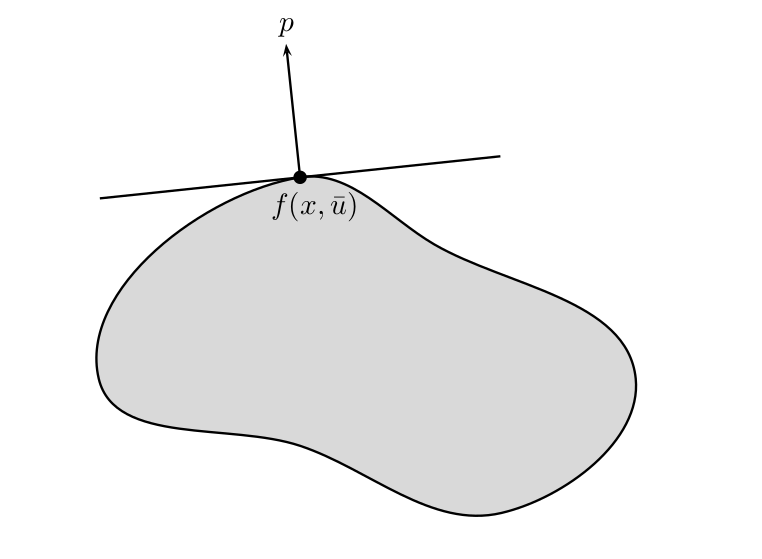
\includegraphics[width=\linewidth]{imgs/512-514.png}
	\caption{In order to maximize the Hamiltonian, the control should be such that $f$ has the maximum projection in the direction of $p$.}
	\label{fig-5.2}
\end{figure}

\subsection{Controlled trajectories and boundary of the reachable set}
The following very important theorem tell us some important things. The first one is that if in the end (at $t_1$) the trajectory lies on the boundary of the reachable set, then there exists an adjoint response that maximizes the Hamiltonian for any instant in $\tzto$ with that control (or, better to say, in the Lebesgue points for $f$ in that interval). Thus, the control is a candidate for optimality since it maximizes the Hamiltonian. \\
%is it optimal for shure, se massimizza l'hamiltoniana, o e' solo un candidato (cioè è una condiz necessaria ma non sufficiente?)??????

\begin{teo}
	Let us have the usual control system, initial condition and time interval, a control $\mu_*\in\admContr{\tzto}$, and $\xi(\mu_*,x_0,t_0,t_1)$ (abbreviate $\xi(\mu_*,x_0,t_0,\cdot)$ simply with $\xi_*(\cdot)$). If $\xi_*(t_1) \in bd(\reachSetMath{t_1})$ then \lista{
	\item there exists an adjoint response $\lambda_*:\tzto\fd\R^n$ for $\Sigma$ for the controlled trajectory $(\xi_*,\mu_*)$ such that 
	\item $H_\Sigma(\xi(\mu_*,x_0,t_0,t),\lambda_*(t),\mu_*(t))=H_\Sigma^{max}(\xi(\mu_*,x_0,t_0,t),\lambda_*(t))$ for almost every $t\in\tzto$
}
	\label{5-16}
	\label{T10}
\end{teo}

\begin{proof}
		Since $\xi_*(t1)$ is on the boundary of the reachable set, then there exists a sequence $\{x_j\}$ in $\chi\backslash closure(\reachSetMath{t_1})$ that converges to that point. Now, let's take another sequence $v_j=\frac{x_j-\xi_*(t_1)}{||x_j-\xi_*(t_1)||}$. Since this sequence lies on the unitary sphere in $R^{n}$ and this set is compact, there exists a converging subsequence, that converges to $v_0$.\\
	We now claim that $v_0\notin int(K(\mu_*,x_0,t_0,t_1))$:\\\\
	\begin{minipage}{0.07\linewidth}
		 \mbox{}
	\end{minipage}
	\begin{minipage}{0.9\linewidth}
		 Supposing that $v_0$ lies in the internal part of the cone, then there exists a sufficiently large $N$ such that, for $j>N$, every $v_j$ lies in the internal of the cone. Theorem \ref{5-10} applies then to this vector.\\
		 Obviously, if $v_j$ lies in the internal of the cone $A$, also $\alpha v_j,\alpha>0$ does.\\
		 Now, since $\{x_j\}$ converges to $\xi_*(t1)$, we can also take that $N$ so that it holds true  $||x_j-\xi_*(t_1)||<\frac{1}{2}r$ for every $j$.\\
		 Since $\alpha v_j\in int(A), \alpha v_j\in A$. We can rescale each $v_j$ such that its module is no longer one, but $||x_j-\xi_*(t_1)||$. Thus, $\xi_*(t1)+\alpha v_j=x_j$, and because of theorem \ref{5-10}, $x_j\in$\reachSet{t_1}, thus violating the hypothesis $\{x_j\}\subset\chi\backslash closure(\reachSetMath{t_1})$.\\
		 
%		 By re-scaling each $v_j$ such that its module is no longer one, but $||x_j-\xi_*(t_1)||$, we then obtain that there is a ball surrounding each one of this vector, which lies in the internal part of  $A$. We must remark that this module is now $<\frac{r}{2}$. If it happens that the radius of this ball is big enough so that $\underset{v\in ball_j}{max}||v||\geq r$, we can just re-scale the ball so it doesn't happen.\\
%		 We can then apply the last part of the theorem \ref{5-10}, and say that there is a whole neighbourhood of $x_j$ contained in the reachable set, thus negating the hypothesis $\{x_j\}\subset\chi\backslash closure(\reachSetMath{t_1})$.
	\end{minipage}\\
	Given this, a topological result states that there exists a separating hyperplane $P(t_1)$ such that vector $v_0$ is contained in a half-space and the cone is contained in the other one.\\
	Now take a the vector called $\lambda_*(t_1)$ orthogonal to $P(t_1)$ lying in the half space not containing the cone, and thus \[\langle \lambda_*(t_1),v\rangle\leq0;\text{\space\space\space}v\in K(\mu_*,x_0,t_0,t_1).\]
	To conclude, we just need to take the unique adjoint response that has the value $\lambda_*(t_1)$ at time $t_1$, and use the preceding theorem \ref{5-13}: the supporting hyperplane for the cone exists a certain instant, so there exists an adjoint response that maximizes the Hamiltonian with the given control.
\end{proof}

\paragraph{Interpretation}
In the following figures we can have a deeper insight of the passages and geometrical constructions behind this theorem. In the left one from Figure\ref{fig-5.3} one can see that the adjoint response points somehow "outside" of the reachable set. Indeed, if the objective is staying on the boundary of the expanding reachable set, it sounds logical to choose a control, and thus an $f(\xi,\mu)$ that "points outside the reachable set, as much as it can". This effort is represented in the maximization of the Hamiltonian,  which is by the maximization of the projection of the possible $f$ and $\lambda$, as depicted in Figure \ref{fig-5.2}. \\
Important remark:the hyperplane actually separates the vector $v_0$ from the cone $K$, so the it does not have to be tangent to the reachable set, as seen in the central part of the figure.\\
Finally, the last of the three figures shows us the evolution of the adjoint response, of the separating plane $P$ (which are guaranteed to exists in the past instants) and of the dotted trajectory.

\begin{figure}[h]
	\centering
	\begin{subfigure}[b]{0.25\linewidth}
		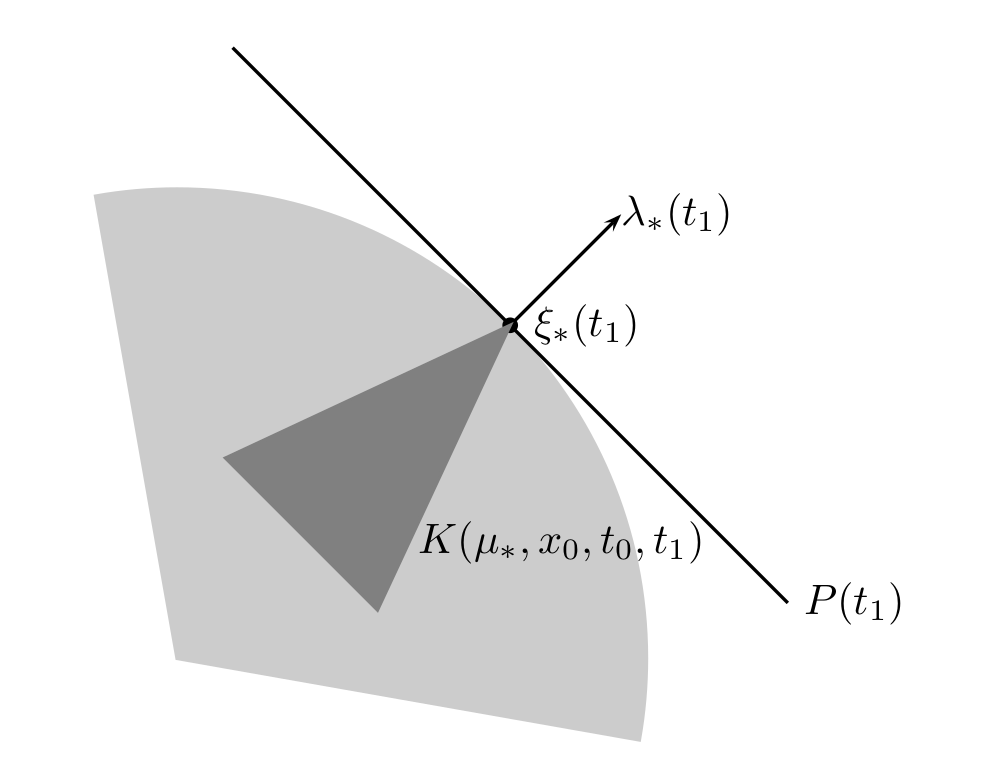
\includegraphics[width=\linewidth]{imgs/5-3-L.png}
		\caption{"Zoom" on the cone, part of the reachable set and final point of the trajectory at the final instant.}
	\end{subfigure}
	\begin{subfigure}[b]{0.25\linewidth}
		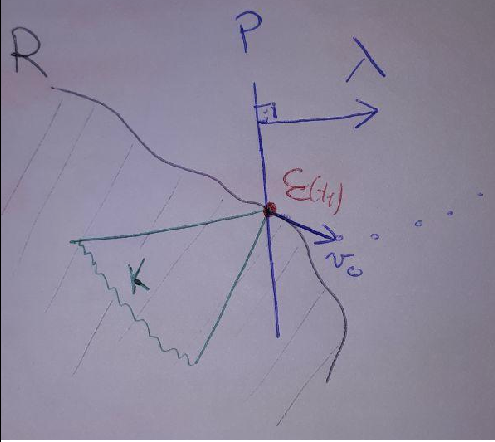
\includegraphics[width=\linewidth]{imgs/5-3-C.png}
		\caption{The separating hyperplane must not be necessarily tangent to the reachable set.}
	\end{subfigure}	
	\begin{subfigure}[b]{0.25\linewidth}
		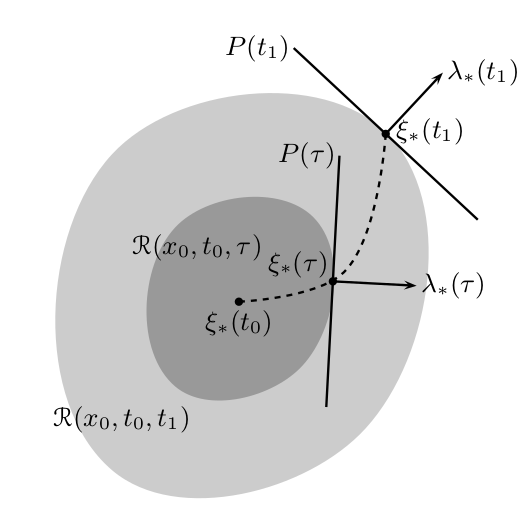
\includegraphics[width=\linewidth]{imgs/5-3-R.png}
		\caption{Depiction of the situation at two different instants, the final one and one intermediate, $\tau$.}
	\end{subfigure}	
	\caption{\mbox{}}
	\label{fig-5.3}
\end{figure}

There is a last theorem for this section, which states that once a system is fallen from the border of the reachable set, it remains in its internal for all the successive instants. Basically, in a crowd of runners where everybody runs at the (same and uniform) maximum speed, once a runner diminishes the speed for an amount of time that is not Lebesgue-neglettable, it will fall inside the crowd, and won't be able to return on the border anymore. 
\\\\\\
\subparagraph[5.17]{Trajectories in the interior of the reachable set remain in its interior}\mbox{}\\
\begin{teo}
	Let's have the usual control system, initial condition, time interval and admissible control. If, for a certain instant $\tau\in[t_0,t_1)$ it happens that $\trajWinCondMath{\tau}\in int(\reachSetMath{\tau})$ then\trajWinCond{t}$\in int(\reachSetMath{t})$ for all $t\in(\tau,t_1]$.
	\label{5-17}
	\label{T11}
\end{teo}

\subsection{Extended system, extended reachable set and optimal trajectories}
Before stating the penultimate theorem, we briefly define one last object, the extended system. It is just the extension from n to n+1 dimensions for the state of the system, where the new, 0-th dimension is the value of the cost function so far.

\subparagraph[6.1]{Definition: Extended System} Let $L$ be a Lagrangian for control system \controlSystem. We define the \grass{extended system} as $\hat{\Sigma}=(\hat\chi,\hat{f},U)$ just by asking that \lista{
	\item $\hat\chi=\R\times\chi$,
	\item $\hat f((x^0,x),u)=(L(x,u),f(x,u))$.
}
Note that now the equations governing the extended system are 
\begin{gather*}
	 \dot{\xi}^0(t)=L(\statot,\mut)\\
	\statotdot=f(\statot,\mut)\\
	\implies\\
	\xi^0(\tau)=\int_{t_0}^{\tau}L(\statot,\mut)dt.
\end{gather*}
This is precisely the cost function.\\
There now will be an important theorem, that lies an important layer in the proof of the principle. In fact, so far, the optimality of a trajectory has always been related to the maximization of an Hamiltonian, as is stated in the proof of the principle. But, looking deeper into the previous theorems, the maximization of the Hamiltonian just ensures that the trajectory lies on the boundary of the reachable set (on the "frontier of runners", so to say). The fact that a trajectory runs through the state space as fast as possible possible has nothing to do, a-priori, with the paid cost associated to that controlled trajectory. 


\paragraph[6.2]{Optimal trajectories lie on the boundary of the extended reachable set}
\begin{teo}
	Let $L$ be a Lagrangian for control system \controlSystem, $\szm,\som\subset\chi$ be sets, and suppose that $(\xi_*,\mu_*)$ is a solution to the fixed interval problem (which is, $(\xi_*,\mu_*)\in\mathfrak{P}(\Sigma,L,\szm,\som,[t_0,t_1])$, then $\hat{\xi}_*(t_1)\in boundary(\extReachSetStarMath{t_1})$.
	\label{6-2}
	\label{T12}
\end{teo}
\begin{proof}
 Since $(\xi_*,\mu_*)\in\mathfrak{P}(\Sigma,L,\szm,\som,[t_0,t_1])$, then the corresponding extended trajectory has the obvious property that the cost $\xi^0(t_1)$ is the lowest possible among all the possible controlled arcs \controlledTraj\space that steer the system from $\xi_*(t_0)\text{ to }\xi_*(t_1)$. So given the set of possible costs , the first element of $\hat{\xi}_*(t_1)$ is obviously on its boundary (at least, as long as the trajectories are L-acceptable, which is, the cost function is finite). This must then imply that also $\hat{\xi}_*(t_1)$ is on the boundary of the extended reachable set: let's take a neighbourhood of $\hat{\xi}_*(t_1)$ in the extended state space $\hat{\chi}$. Any neighbourhood will then contain points of the form $(c,\xi_*(t_1))$ with $c<\xi_*^0(t_1)$. But those points, with a cost which is littler than the minimum one, are not in the extended reachable set by hypothesis, since the controlled trajectory  $(\xi_*,\mu_*)$ is optimal. So, since there is no neighbourhood of $\hat{\xi}_*(t_1)$ contained in \extReachSetStar{t_1}, this point must lie on the boundary, as wanted.
\end{proof}
%To see if this is true. Certainly, it is not useful,
%The fact that $\hat{\xi}_*(t_1)$ is on the boundary of the extended reachable set implies that the trajectory $\xi(t_1)$ is on the boundary of \reachSet{t_1}, thus implying the bond with cost-wise optimality and being on the boundary of the reachable set, which is an Hamiltonian-wise optimality. Indeed, it will be used in the following theorem.


\subsection[6.3]{Adjoint response, Hamiltonian and maximum principle}
Finally, we will now prove the points 1 to 3 in the statement of the principle. 

\begin{teo}
	Let $L$ be a Lagrangian for control system \controlSystem, $\szm,\som\subset\chi$ be sets, and suppose that $(\xi_*,\mu_*)$ is a solution to the fixed interval problem (which is, $(\xi_*,\mu_*)\in\mathfrak{P}(\Sigma,L,\szm,\som,[t_0,t_1])$), then there exists an absolutely continuous map $\lambda_*:\tzto\fd\R^n$ and a number $\lambda_*^0\in\{-1,0\}$ with the following properties:
\begin{enumerate}
	\item either $\lambda_*^0=-1$ or $\lambda_*(t_0)\ne0$,
	\item $\lambda_*$ is an adjoint repsonse for $(\Sigma,\lambda_*^0L)\text{ along }(\xi_*,\mu_*)$,
	\item $H_{\Sigma,\lambda_*^0L}(\xi_*(t),\lambda_*(t),\mu_*(t))=H_{\Sigma,\lambda_*^0L}^{max}(\xi_*(t),\lambda_*(t))$ for almost every $t\in[t_0,t_1]$.
\end{enumerate}
	\label{6-3}
\end{teo}

\begin{proof}
	First, we observe that the vector $(-1,0)\in\R\times\R^n$ cannot lie in the interior of the extended tangent cone \extFixIntTanCone{t_1}. If this were not the case, by means of theorem \ref{5-10}, there would be points $(a^0,a)\in$ \extReachSetStar{t_1} at a lower cost, whose state is the same, at the same time, as the optimal trajectory ($a=\xi_*(t_1)$). This would violate the optimality of $(\xi_*,\mu_*)$.\\
Since this vector does not lie in the interior of \extFixIntTanCone{t_1}, there exists a separating hyperplane $\hat P(t_1)$ between this cone and the vector. \\
Take a vector $\hat{\lambda}_*(t_1)$ orthogonal to $\hat P(t_1)$, in the half space not containing the cone. This implies 
\gatherNo{
	\langle \hat{\lambda}_*(t_1),(-1,0) \rangle\ge0,\\
	\langle \hat{\lambda}_*(t_1),\hat{v}\rangle\le0;\text{\space\space\space     }\hat{v}\in\extFixIntTanConeMath{t_1}
}
This implies then that $\hat{\lambda}_*^0(t_1)\leq0$.\\
Define then $\hat{\lambda}_*$ as the adjoint response whose value at $t_1$ is equal to $\hat{\lambda}_*(t_1)$.\\
From the equations for the adjoint response \eqref{adjoint-equation} we obtain that $\dot{\lambda}_*^0(t)=0$. This is because since $\hat f$ does not depend on $x_0$, then the Jacobian matrix $\Dderarg{1}\hat f$ has the first column $0$, and thus the transposed matrix has the first row of zeros. This is of course by imagining the (extended) adjoint response as a coloumn vector.\\
So $\lambda_*^0(t)=0$ is constant and nonpositive. So, if $\lambda_*^0(t)\neq0$, we can rescale the whole extended adjoint response so that $\hat{\lambda}_*$ becomes $\frac{\hat{\lambda}_*}{-(\lambda_*^0)}$, so that now $\lambda_*^0$ is either 0 or -1.\\
The Hamiltonian for the extended system is very similar to the extended Hamiltonian for the system (plus the Lagrangian):
\gatherNo{\hat{H}_{\hat{\Sigma}}\left((x^0,x),(p^0,p),u\right)=\langle p,f(x,u)\rangle+p^0L(x,u)=H_{\Sigma,p^0L}(x,p,u)}
Now, since the trajectory is optimal, by \label{YET-ANOTHER-REFERENCE5} virtue of theorem \ref{6-2}, it lies on the boundary of the extended reachable se at time $t_1$. Then it hold s true that $H_{\Sigma,p^0L}(\xi_*(t),\lambda_*(t),\mu_*(t))=
H_{\Sigma,p^0L}^{max}(\xi_*(t),\lambda_*(t))$ for almost every $t\in\tzto$.\\
The fact that at least one between $,\lambda_*(t_0)$ and $\lambda_*^0$ is not zero derives from the linearity of the adjoint equation. 
\end{proof}


%Actually, the last theorem used deals with the boundary of the reachable set and not extended system, but it is enough to imagine that the extended system is just a normal system with an added dimension. 